\documentclass[conference]{IEEEtran}
\usepackage{graphicx,amsmath}
\usepackage{psfrag}
\usepackage{multirow}%ʹ�ö������
\hyphenation{op-tical net-works semi-conduc-tor IEEEtran}


\IEEEoverridecommandlockouts
\usepackage{color}
\usepackage{geometry}
\geometry{a4paper,top=2.5cm,bottom=3.5cm,left=1.3cm,right=1.3cm}
\begin{document}

% paper title
\title{Energy-Efficient Power and Subcarrier Allocation for OFDMA Systems with Value Function Approximation Approach}


% author names and affiliations
% use a multiple column layout for up to three different
% affiliations
\author{\authorblockN{Kai Bi, Qinghai Yang, FengLin Fu \thanks{*This research was supported in part by the RCUK for the UK-China Science Bridges Project: R\&D on (B)4G wireless mobile communications, by the National Research Foundation of Korea (No. 2010-0018116), NSF of China (61001127, 60832001)}}
\authorblockA{State Key Laboratory of ISN, \\School of Telecomm. Engineering, \\Xidian University, No.2 Taibainan-lu,\\ Xi'an,
710071,
Shaanxi,China. \\
Email:qhyang@xidian.edu.cn} \and
\authorblockN{Kyung Sup Kwak}
\authorblockA{Graduate School of IT \\and Telecomm., Inha
University, \\{\#}253 Yonghyun-dong, Nam-gu,\\ Incheon, 402-751,
Korea. \\Email: kskwak@inha.ac.kr}%\thanks{ddd}

}

\maketitle

\begin{abstract}
In this paper, we conceive an energy-efficient power and subcarrier allocation scheme for downlink OFDMA systems under average delay constraints. The services associated with multi-users have different packet arrivals and delay requirements. The problem of dynamic power and subcarrier allocation is formulated as a constrained Markov decision process (CMDP) with control actions based on the joint states of channel state information (CSI) and the queue state information (QSI). An online learning algorithm is developed for solving the CMDP problem with the aid of stochastic approximation and the value function approximation approach.



\end{abstract}

\begin{keywords}
Energy-efficient, resource allocation, constrained Markov decision process, stochastic approximation, value function approximation.
\end{keywords}

% no keywords

% For peer review papers, you can put extra information on the cover
% page as needed:
% \begin{center} \bfseries EDICS Category: 3-BBND \end{cen['ter}
%
% for peerreview papers, inserts a page break and creates the second title.
% Will be ignored for other modes.
\IEEEpeerreviewmaketitle

\section{Introduction}
% no \PARstart
With the rapid development of wireless systems in terms of the number of subscribers and applications, two key design challenges lie in the power-efficient transmission of portable handsets, as well as the delay-sensitive multimedia transmission applications such as video conference, remote teaching/training, etc. Both of these two challenges require highly efficient scheduling and resource allocation schemes.

Many efforts have been made on the cross-layer optimization of power and subcarrier allocation for orthogonal frequency division multiple access (OFDMA) systems. The traditional view of considering the energy-efficient and delay-sensitive applications were to treat the wireless system as a layered network \cite{1}. In the single user scenario, the pioneer work of \cite{2} investigated the energy efficient delay-constraint cross-layer scheduling scheme under the channel variation and buffer dynamics. Following the model of Berry-Gallager, the energy efficient transmission was investigated under the average delay constraint in the constrained Markov decision process (CMDP) framework [3-5]. Literature \cite{5} analyzed the structural properties of optimal transmission policies over a randomly varying channel. A stable online algorithm was developed in \cite{6}, which was interpreted as \lq\lq one component at a time\rq\rq, via introducing a middle state called post-decision state. The work of \cite{7} extended the model in \cite{6} to a single-cell multiuser wireless uplink system and provided the convergence analysis and queue stability proof.
	
In this paper, we investigate an energy-efficient resource allocation with value function approximation under average delay constraint. It proves that the post-decision value function for the problem of the energy efficient scheduling under average delay constraint is convex on the backlog at BS. And the post-decision value function is approximated using the piecewise linear function to attain quick convergence.

\begin{figure}
\centering
\includegraphics[width=2.6 in]{fig1.eps}
\label{fig1}\caption{System model}
\end{figure}

\section{System Model and State Definition}
\subsection{System Model}
We consider an OFDMA downlink system with $M$ users, $N_F$ subcarriers, and one base station (BS), as depicted in Fig. 1. BS manages $M$ queues, which are associated with $M$ users, respectively. In a non-homogenous user scenario, different application streams may have different arrival rates, and delay requirements. The subcarrier and power allocation is performed with respect to the effects of both channel state information (CSI) and queue state information (QSI).

We assume the channel is time-varying but keeps constant over the interested time interval. We use a finite-state Markov model to describe the fading channel. The corresponding one-step transition probability is computed by the method in \cite{9}.

We assume that, the packets from higher layers arrive at the end of each slot and their arrivals of the packets are independently identically distributed (i.i.d). The packet arrival process and the channel state evolution process are assumed to be stationary and independent. The packets of different users are stored in the corresponding queues at BS for transmission. We denote $q_i^{t} $ and $U_i^t $ as the queue length in the buffer of user $i$ and the number of transmitted packets at time slot $t$. If the number of data arrivals is $A_{i}^{t+1}$, the queue length at the next time slot can be expressed as:

\begin{equation}
\label{eq1} q_{i}^{t+1} =q_i^{t} -U_i^{t} +A_{i}^{t+1}.
\end{equation}

Supposing the buffer size is $N_Q$ in a practical system, the queue length at time $t+1$ is $q_{i}^{t+1} =\min (q_i^{t} -U_i^{t} +A_{i}^{t+1} ,N_Q)$. If $N_Q$ is large enough, the buffer overflow can be neglected. Next, let denote $\bar {q}$ and $\bar {D}$ as the average queue length and average delay, respectively. According to Little's Theorem, it holds $\bar {q}=\bar {a}\bar {D}$ where $\bar {a}$ is a parameter. That is, the delay constraint of each user can be mapped to that of the queue length.

\subsection{State Definition}
The cardinality of the set QSI is $L=(N_Q+1)^M$, which grows exponentially with $M$. Denote the system state as: $s^t =\left({s_1^{t}, s_2^{t}, \cdots, s_L^{t} } \right)$ with $s_i^{t} =\left( {q_i^{t} ,h_i^{t} } \right)$, where $h_i^{t} $ represents the channel gain of user $i$ at time slot $t$. The joint allocation scheduling policy of $M$ queues is stated as $\pi^t =({\pi_{1,1}^{t}, \pi_{1,2}^{t}, \cdots, \pi_{1,N_F}^{t}};\cdots;{\pi_{i,1}^{t}, \pi_{i,2}^{t}, \cdots, \pi_{i,N_F}^{t}};\cdots;{\pi_{M,1}^{t},} \\{\pi_{M,2}^{t}, \cdots, \pi_{M,N_F}^{t}})$. $\pi _{i,n}^{t} $ is an indicator that indicates whether queue $i$ gets the $n$-th subcarrier at time slot $t$. $\pi_{i,n}^{t} =1$ means queue $i$ gets the $n$-th subcarrier at current time slot, and $\pi_{i,n}^{t} =0$ represents waiting for transmission in the next slot. The queue length in the next time slot is affected by the current queue length and the number of packets to be transmitted. We assume the channel state acts as an ergodic Markov chain and inevitably transits into another state at the next time slot. Thus, it can be formulated as a CMDP problem.

\makeatletter
\newcommand{\Extend}[5]{\ext@arrow 0099{\arrowfill@#1#2#3}{#4}{#5}}
\makeatother

We denote the state transition from time $t$ to $t+1$ by
$s^t\rightarrow s^{t+1}$, represented by:
\[
s_{i}^t=(q_{i}^t,h_{i}^t)\Extend{-}{-}{>}{}{y^{t}_i}
s_{i'}^{t+1}=(q_{i'}^{t+1},h_{i'}^{t+1}).
\]

Assuming that the queue
length and the channel fading are independent of each other, the
probability of state transition is expressed by:
\begin{eqnarray}
\label{eq2}
p(s_{i'}^{t+1}|s_{i}^t,y_{i}^t)
&=&p(q_{i'}^{t+1}|q_{i}^t,y_{i}^t)p(h_{i'}^{t+1}|h_{i}^t)\nonumber\\
&=&p(A_{i}^{t+1})p(h_{i'}^{t+1}|h_{i}^t).
\end{eqnarray}

\section{Problem Formulation}

Given the defined the system state $s_i^{t} =\left( {q_i^{t} ,h_i^{t} } \right)$, the transmitter may adjust the transmit power and subcarrier allocation according to a stationary policy $\pi^t =\left( {\pi_1^{t} ,\pi_2^{t} ,\cdots ,\pi_{N_F}^{t} } \right)$. A transmission policy $\pi^t $ is a mapping from a system state $s^t$ to a power control and subcarrier allocation actions. A policy $\pi^t $ is called feasible if the allocation actions satisfy the average total transmit power constraint and the subcarrier assignment constraint. Power allocation should satisfy:
\begin{equation}
\label{eq3} { \sum\limits_{i=1}^{M}\sum\limits_{n=1}^{N_F}{E[P_{i,n}]}\leq P_0 , ~~~ P_{i,n}\ge 0,  }
\end{equation}
where $P_0$ denotes the maximum power that allowed at BS.

The subcarrier allocation should satisfy the constraint:
\begin{equation}
\label{eq4}{ \sum\limits_{i=1}^{M} \pi_{i,n} = 1 ,~~~ \forall n \in \{1, N_F \} }.
\end{equation}

We write the infinite horizon discounted power expenditure that queue $i$ consumed:

\begin{equation}
\label{eq3}   P_i=\mathcal{E}\left[{\sum\limits_{t=1}^\infty {\alpha^tP(U_i^{t} ,h_i^{t} )} } \right].
\end{equation}

Similarly, the average delay of queue $i$ is expressed as:
\begin{equation}
\label{eq4}  Q_i=\mathcal{E}\left[ {\sum\limits_{t=1}^{\infty}{\alpha^tq_i^{t} } } \right],
\end{equation}
where $\alpha $ is the discounted factor in the range of [0, 1).

Accordingly, the problem may be formulated as:
\begin{equation}
\label{eq5}
\begin{array}{l}
 \min \mbox{ } {P}_i\\
  \mbox{s. t. }\enspace {Q}_i \le \zeta_i,\enspace i=1,\cdots ,M \end{array}
\end{equation}
where $ \zeta _i$ denotes the maximum delay that the $i$-th user could tolerate.

\section{Allocation Policy}

The resource allocation controller computes which queue will be allocated one or more subcarriers for transmission based on CSI at each time slot. The allocation decision in a time slot affects the buffer occupancy of all the queues in future slots, in other words, the average delay of everybody. At each time slot, the controller calculates the transmission rate based on QSI and power expenditure for each queue online based on multiple traffic's delay  constraints. The rate for each queue is denoted as $y_i^{t} $. Combining this rate with CSI at current slot, we can compute the corresponding power expenditure $P_i^{t}$. In this way, the controller analyzes all information and finally makes the allocation decision. In the next time slot, the controller remake the allocation decision based on the decision made at the last time slot as well as both the new CSI and QSI.

\section{Online Learning with Value Function Approximation}
\subsection{Lagrangian Approach}

We define the utility function as the long-term average power expenditure under average delay constraints. The controller computes the required transmission rate for an individual queue online based not only on the current queue length and channel state but also on the future likely states. While introducing Lagrange factor, the constrained problem can be converted to a non-constrained problem.

It is equivalent to maximize:
\begin{equation}
\label{eq7}
\begin{array}{ll}
L(\lambda_{i}^t,q_{i}^t,h_{i}^t,y_{i}^t)=
\mathcal{E}\Bigl{[}\sum\limits_{t=1}^{\infty}\alpha^t\times\\
 \big{[}P(h_{i}^t,y_{i}^t)-\lambda_{i}^t(Q(q_{i}^t,y_{i}^t)-\zeta_{i})\big{]} \Bigr{]},
\end{array}
\end{equation}
where $y_{i}^t$ is the required transmission rate for queue $i$. For a certain $\lambda_{i}^t$, this problem is a non-constrained MDP problem.
Depriving the delay deadline $\zeta_{i},i=1,\cdots,N$, according to \cite{10}, the non-constrained Markov decision process problem can be solved by:
\begin{equation}
\label{eq8} \mu^{*}_{\zeta}(s_0) =\min_{\lambda_{i}^t \geq
 0}\max_{y_{i}^t\in
 \Phi}N_{y_{i}^t,\lambda_{i}^t}(s_0)+\lambda_{i}^t\zeta_{i},
\end{equation}
where the so-called normal state value function is expressed as:
\begin{equation}
\label{eq9}
\begin{array}{ll}
N_{y_{i}^t,\lambda_{i}^t}(s_0)=\mathcal{E}\Bigl{[}\sum\limits_{t=1}^{\infty}\alpha^t\times\\
\big{[}P(h_{i}^t,y_{i}^t)-\lambda_{i}^t(Q(q_{i}^t,y_{i}^t)\big{)}|s_0\big{]}\Bigr{]}.
\end{array}
\end{equation}

Further based on dynamic optimization theory, it is equivalent to solve:
\begin{equation}
\label{eq10}
\begin{array}{ll}
N_{i^*,\lambda_{i}^t}(s)=\min\limits_{y_{i}^t\in \Phi_{i}}\biggl{[}
P\big{(}y_{i}^t(s),h_{i}^t\big{)}-\lambda_{i}^t Q\big{(}q_{i}^t,y_{i}^t(s)\big{)}\\
+\alpha\sum\limits_{s'}p\big{(}s'|s,y_{i}^t(s)\big{)}N_{i^*,\lambda_{i}^t}(s')\biggr{]},\forall s.\end{array}
\end{equation}

\subsection{Structural Analysis of Post-Decision State Value Function}

The classic approaches to solve CMDP are based value iteration, and policy iteration, etc, in which the knowledge of a prior probability is necessary to be known. However, this requires the probability distributions of the arrivals and channel states, which are generally unknown in practical communication system. Meanwhile, when determining the optimal solution, the optimal Lagrange factor is necessary to be found.

From \cite{6}, after a post-decision state is introduced, the conditional expectation and the maximization operator can be swaped. Besides, the prior probability information is separated from the normal state value function. Thus, we can represent the normal state value function through post-decision state function explicitly. The following analysis shows that the post-decision state function is coupled with the normal state value function.

The definition of the post-decision state is given by:
\begin{equation}
\label{eq11}
{s}^t_{i}=({q}_{i}^t,{h}_{i}^t)=(q_{i}^t-y_{i}^t,h_{i}^t).
\end{equation}

The queue length denotes the buffer occupancy after the data transmitted and before the new data comes. The post-decision channel state inherits the same as the current one.

\textbf{Remark 1}: Due to the competition for the common channel, not all the requested transmission $y_{i}^t$ is guaranteed, so the actual queue length variation follows:
${q}^t_{i}=q_{i}^t-\sum\limits_{n=1}^{N_F}\pi_{i,n}^ty_{i}^t$;

The post-decision state value function $V_{*,\lambda}(q,h)$ represents the optimal long-term utility starting from the post decision state,
\begin{equation}
\label{eq13} V_{*,\lambda}(q,h)=\sum_A\sum_{h'\in
H}p(A)p(h'|h)N_{*,\lambda}\big{(}(q+A),h'\big{)}.
\end{equation}

The corresponding optimization problem can be expressed as:
\begin{equation}
\begin{split}
\label{eq14} N_{*,\lambda}(q,h)=\min_{0\leq y\leq q}\bigl{[}{P(h,y)}-\lambda Q(q,y)\\+\alpha V_{*,\lambda}(q-y,h)\bigl{]}.
\end{split}
\end{equation}

Based on the relative value iterative algorithm, we can update the components of post-decision state function in a \lq\lq one component at a time\rq\rq~way as \cite{6}. However, this approach requires relatively large storage space. This prompts us to analyze the structure properties of the optimal required transmission rates. Meanwhile, we suppose the post-decision state
value function preserves some properties as the function in \cite{8}.

The following  process shows the properties of the post-decision state value function. From (\ref{eq13}), we note that to compute the post-decision state value function, it is necessary to know the underlying dynamics, i.e. the distribution of the traffic arrivals and the channel transition probability; that is, to perform the expectation on all possible states over the normal-state value function (c.f. Eq.(10)). For simplicity, the expectation can be replaced via the averaging over time. The update of the post-decision state value function is given by:
\begin{equation}
\label{eq15}
\begin{array}{ll}
V_{t,\lambda}(\tilde{q},h^{t-1})=(1-\beta^t)V_{t-1,\lambda}(\tilde{q},h^{t-1}) \\\\
\verb+           ++\beta^tJ_{t,\lambda}((\tilde{q}+A),h^t),\forall
\tilde{q}
\\\\
V_{t,\lambda}(\tilde{q},\tilde{h})=V_{t-1,\lambda}(\tilde{q},\tilde{h}),\forall
\tilde{q},\tilde{h}\neq h^{t-1}.
\end{array}
\end{equation}

Similar to the analysis in \cite{8}, some results on the post-decision state value function are developed given the objective and constraints in the paper. Here, we shall approximate the
value function using piecewise linear function \cite{11}.

\textbf{Proposition}: The maximum transmission rate for each queue $y_{i}(q,h),i=1,\cdots,N$ is non-decreasing with $q$ and the post-decision state value function
$V_{*,\lambda}(\tilde{q},\tilde{h})$ is convex of $q$.

\proof
First, we construct the power function and the delay function
as $P(h,y)=({\sigma^2}/{|h|^2})(2^y-1)$ and
$Q(q,y)=q-y $, respectively.
The optimization function is given by:
\begin{equation}
\begin{split}
\label{eq16} N_{\ast,\lambda}(q,h)=\max\limits_{0\leq y\leq q}\Bigl{[}-P(h,y)-\lambda Q(q,y)\\+\alpha V_{*,\lambda}(q-y,h)\Bigr{]}.
\end{split}
\end{equation}

Subsequently, we demonstrate $-P(h,y)-\lambda Q\left( {q,y} \right)$ satisfies the
definition of supermodularity.

\textbf{Supermodularity} (definition): For any ${y}'\ge y,\enspace {x}'\ge x$, if the following
expression holds:
\begin{equation}
f\left( {{x}',{y}'} \right)-f\left( {{x}',y} \right)\ge f\left(
{x,{y}'} \right)-f\left( {x,y} \right).
\end{equation}
Then, the function $f:X\times Y\to R$ is a super modularity on the pair
of $\left( {x,y} \right)$.

Let $f\left( {q,y} \right)=-P\left( {h,y} \right)-\lambda Q\left( {q,y}
\right)$, for any $q\ge {q}',y\ge {y}'$. Then, it yields
\begin{displaymath}
\begin{array}{ll}
f(q',y')-f(q',y)\\\\ \displaystyle=-P(h,y')-\lambda Q(q',y')-[-P(h,y)-Q(q',y)]\verb+   +(*1)\\\\
=\displaystyle
-\frac{\delta^2}{|h|^2}(2^{y'}-1)+\frac{\delta^2}{|h|^2}(2^{y}-1)-\lambda(q'-y')+\lambda(q'-y),
\end{array}
\end{displaymath}
\begin{displaymath}
\begin{array}{ll}
f(q,y')-f(q,y)\\\\=-P(h,y')-\lambda Q(q,y')-[-P(h,y)-Q(q,y)]\verb+    +(*2)\\\\
=\displaystyle
-\frac{\delta^2}{|h|^2}(2^{y'}-1)+\frac{\delta^2}{|h|^2}(2^{y}-1)-\lambda(q-y')+\lambda(q-y).
\end{array}
\end{displaymath}

Obviously, $\left( *1 \right)-\left( *2 \right)=0$. Thus, we
verified that $-P(h,y)-\lambda Q\left( {q,y} \right)$ is
supermodularity in pair of $\left( {q,y} \right)$.

Next, we shall show that $V_{m-1,\lambda} \left( {q-y,h} \right)$ is
supermodularity in pair of $\left( {q,y} \right)$ and is also a convex function on $q$.

For any $V_{0,\lambda} \left( {q,y} \right)$, the value iteration
ensures that the post-decision state function converges to the $V_{\ast,\lambda }\left( {q,y} \right)$[8]. Supposing that $V_{0,\lambda} \left({q,y} \right)=q$ and $V_{m-1,\lambda} \left( {q,h} \right)$ is monotonic and convex on $q$, we have
\[
\begin{array}{ll}
V_{m-1,\lambda}(q_1,h)+V^{\lambda}_{m-1}(q_2,h)\\\\ \leq
V_{m-1,\lambda}((1-\eta)q_1+  \eta q_2,h)+V_{m-1,\lambda}(\eta
q_1+(1-\eta)q_2,h),\\\\ \forall \eta\in[0,1].
\end{array}
\] considering
$q'\geq q$, $y'\geq y$ and $q\geq y'$.

 Let
$q_1=q'-y$, $q_2=q-y'$ and $\eta=\displaystyle\frac{y'-y}{q'-q+y'-y}$.
The following two expressions hold:
\[
(1-\eta)q_1+\eta q_2=q'-y'.
\]
\[\eta q_1+(1-\eta)q_2=q-y.
\]
Thus, we obtain
\[
\begin{array}{lll}
V_{m-1,\lambda}(q'-y,h)+V_{m-1,\lambda}(q-y',h)\\\\ \leq
V_{m-1,\lambda}(q-y,h)+V_{m-1,\lambda}(q'-y',h).
\end{array}
\]

Now, we observe that $V_{m-1,\lambda} \left( {q-y,h} \right)$ is
supermodularity in the pair of $\left( {q,y} \right)$.

To demonstrate that $V_{m,\lambda} \left( {q,h} \right)$ is
convex on $q$, we first verify $N_{m,\lambda} \left( {q,h} \right)=\mathop
{\max }\limits_{0\le y\le q} T_{m,\lambda} \left( {q,h,y} \right)$ is convex
on $q$. For any $q_1 $ and $q_2 $, we assume that the optimal scheduling policies
are $y_1 =y^\ast \left( {q_1 ,h} \right)$ and $ y_2 =y^\ast
\left( {q_2 ,h} \right)$. For all $\eta \in \left[ {0,1} \right]$, we have
\[
\begin{array}{ll}
N_{m,\lambda}(q_1,h)+N_{m,\lambda}(q_2,h)\\\\
=-P(h,y_1)-\lambda Q(q_1,y_1)+\alpha V^{\lambda}_{m-1}(q_1-y_1,h)-P(h,y_2)\\\\
 \verb+  +
-\lambda Q(q_2,y_2)+\alpha V_{m-1,\lambda}(q_2-y_2,h)
\\\\ \leq \!\!\!-P(h,\eta
y_1\!+\!(\!1\!-\eta)y_2)\!-\!\!\lambda Q\!\left( \eta q_1+(\!1\!-\!\eta)q_2,\eta
y_1\!+\!(\!1-\!\eta)y_2\! \right)
\\\\ \verb+  + +\alpha
V_{m-1,\lambda}(\eta(q_1-y_1)+(1-\eta)(q_2-y_2),h)
\\\\=T_{m,\lambda}(\eta q_1+(1-\eta)q_2,h,\eta y_1+(1-\eta)y_2)
\\\\ \leq
N_{m,\lambda}(\eta q_1+(1-\eta)q_2,h).
\end{array}
\]

On the hypothesis that $Q\left( {q,y} \right)$ is jointly convex in the pair
of $\left( {q,y} \right)$ (obviously, the hypothesis holds), we know
$N_{m,\lambda} \left( {q,h} \right)$ is convex on $q$. Meanwhile, $V_{m,\lambda}
\left( {q,h} \right)=\sum\limits_A {\sum\limits_{{h}'\in H} {p\left( A
\right)} } p\left( {{h}'\vert h} \right)J_{m,\lambda} \left( {q,h} \right)$.
Thus, $V_{m,\lambda} \left( {q,h} \right)$ is convex on $q$.
\endproof

\subsection{Online Learning Algorithm with Value Function Approximation}

Based on the  above analysis, we know $V_{m,\lambda} \left( {q,h}
\right)$ is convex in the buffer backlog. The normal state value
function $N_{\ast ,\lambda }\left( {q,h} \right)$ can be expressed
by $V_{m,\lambda} \left( {q,h} \right)$ explicitly. We note that if
we derive the expression $V_{m,\lambda} \left( {q,h} \right)$, the
maximum required transmission rate can be easily guaranteed via Eq. (16).
However, the closed-form expression of the
post-decision state value function is still unknown. Literature \cite{11} introduces a
method to approximate the univariate convex function using only
function value evaluations. Thus, we can approximate the
post-decision state value function using piecewise linear function.
Setting a threshold error $\delta _{\max } $, we can adaptively
select the points $\left( {q_1, q_2, \cdots, q_{M_{\delta _{max } }
} } \right)$ to evaluate the value of the post-decision state value
function which is convex in the backlog $q$.

Now, we shall develop the algorithm with value function approximation
approach.

\begin{flushleft} \rule{8.8cm}{0.03em}\end{flushleft}
\begin{enumerate}
\item Initialization: initialize the potential post-decision state value matrix for all channel states and queue lengths, the slot counter $t=0$, post-decision state $\widetilde{s}_0=(q_0,h_0)$, Lagrange factor $\lambda=0$ in the $0$-th regenerative period.

\item At the beginning of the $k$-th regenerative period, determine the new channel state $q_t$ and incoming data $A_{t-1}$ at current time slot and compute the normal state $s_t=(\min(q_{t-1}+A_{t-1},N_Q),h_t)$.
\item Run the system with policy $\pi^t$, judge the current post-decision channel state and approximate the corresponding post-decision state value for all queue lengths at least once using a piecewise linear function.
\item At the beginning of the next regeneration, update the post-decision state value function:
\[\begin{array}{ll}
V^t_{\lambda}(q,h^{t-1})=(1-\beta^t)V^{t-1}_{\lambda}(q,h^{t-1})\\\\
\verb+    + +\beta^{t}N^t_{\lambda}(min(q,+a^{t-1},B),h^t),\forall q.
\end{array}\]
\[V^t_{\lambda}(q,h'')=V^{t-1}_{\lambda}(q,h''),\forall q,h''\neq h^{t-1}
\]
and $N_{t,\lambda}(q,h^t)=\min\limits_{0\leq y\leq
q}\Bigl{[}P(h^t,y)-\lambda Q(q,y)+\alpha
V^{t-1}_{\lambda}(q-y,h^t)\Bigr{]}$.


Compute the optimal required transmission rate based on the current normal state $s_t=(\min(q_{t-1}+A_{t-1},N_Q),h_t)$ through
\[\begin{array}{ll}
&N^t_{\lambda}(q,h)\\
&=\min\limits_{0\leq y\leq q}\Bigl{[}P(h,y)-\lambda Q(q,y)+\alpha
V^{t-1}_{\lambda}(q-y,h)\Bigl{]}.
\end{array}
\]

\item Suppose BS transmits data at the expected transmission rate $y^t_*$.\\
Update the post-decision state
\[
\widetilde{s}^t=(min(q^{t-1}+a^{t-1},B)-y^t_{*},h^t).
\]
Update the Lagrange factor
\[\lambda_{n+1,i}=\max[\lambda_{n,i}+\frac{1}{n}(Q_{n,i}-\zeta_{i}),0].\]

\item If $\lVert {V}^{k+1}_\lambda - V^k_\lambda \rVert < \delta_v$, stop; Otherwise, set k=k+1 and go to step 2 for a new regeneration.
\end{enumerate}
\begin{flushleft} \rule{8.8cm}{0.03em}\end{flushleft}

\textbf{Remark 2:} When implementing this algorithm, we update the
post-decision state function simultaneously for all states while remaining the channel
state $\hat {h}^{t-1}$ unchanged, instead of updating the post-decision state value
function only at current state $\left( {\hat {q}^{t-1} ,\hat {h}^{t-1} }
\right)$. This is known as \lq\lq batch update\rq\rq, which greatly accelerates the
convergence rates for the post-decision state value function.

\section{Simulation Results}

In this section, simulations are provided to illustrate our proposed schemes. The power expenditure function for transmitting the amount of $y$ (in packets) traffic at the channel state $h$ is given by $P(h,y)=\displaystyle\frac{\sigma ^2}{\left| h \right|^2}\left(
{2^{\frac{yl}{W}}-1} \right)$, where $\sigma ^2$ is the variance of the white Gaussian noise, $l$ denotes the packet length and $W$ is the
bandwidth. We assume $\displaystyle\frac{\bar {h}^2}{\sigma ^2}=0.14$ with $\bar {h}$ being the
average channel gain. In the simulation, we assume there are 2 users, 4 subcarriers with total bandwidth 31.25KHZ, $N_Q$= 4 and $\lambda_i$= 80 packet/s.

\begin{figure}[htbt]
\centering
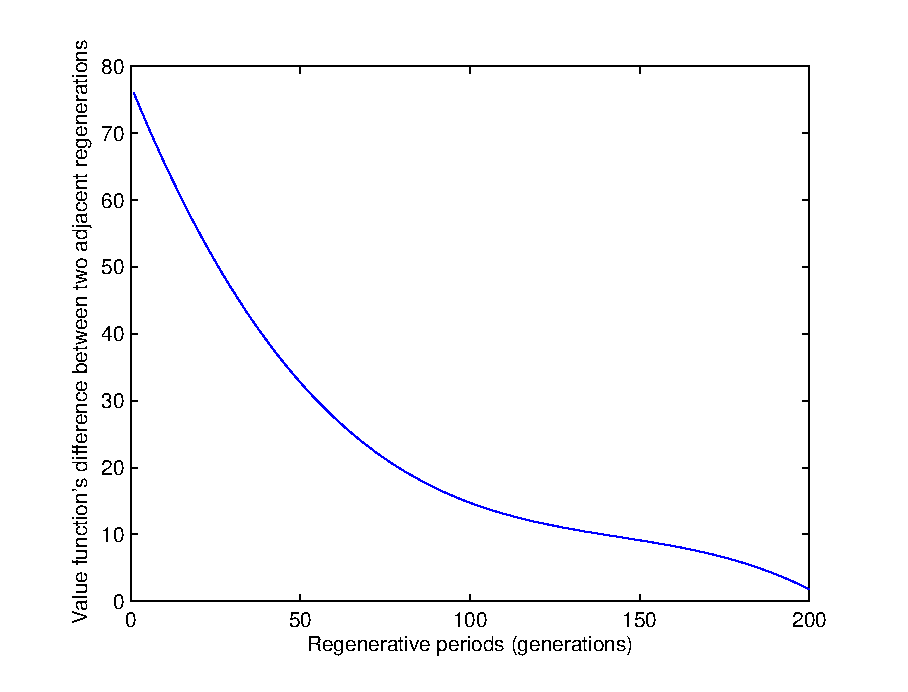
\includegraphics[width=3.5 in]{fig3.eps}
\vspace{-10pt}
\label{fig3}\caption{Graphics trends for $\lVert {V}_\lambda^{k+1}- V_\lambda^k \rVert $ with 200 regenerations by value evaluations.}
\end{figure}

\begin{figure}[htbt]
\centering
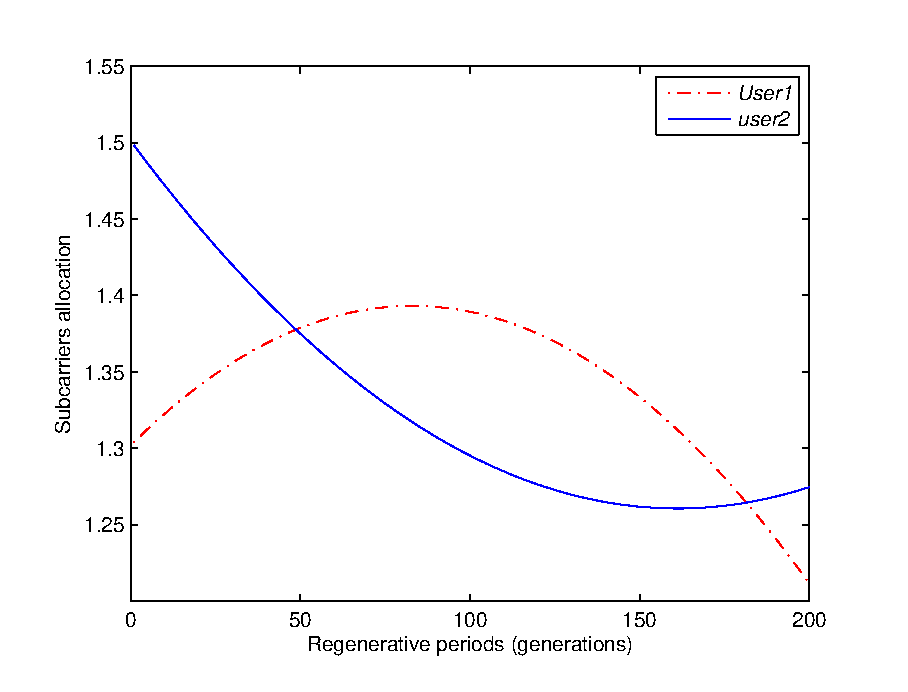
\includegraphics[width=3.5 in]{fig5.eps}
\vspace{-10pt}
\label{fig5}\caption{Average subcarriers allocation versus regenerations periods of the two users.}
\end{figure}

\begin{figure}[htbt]
\centering
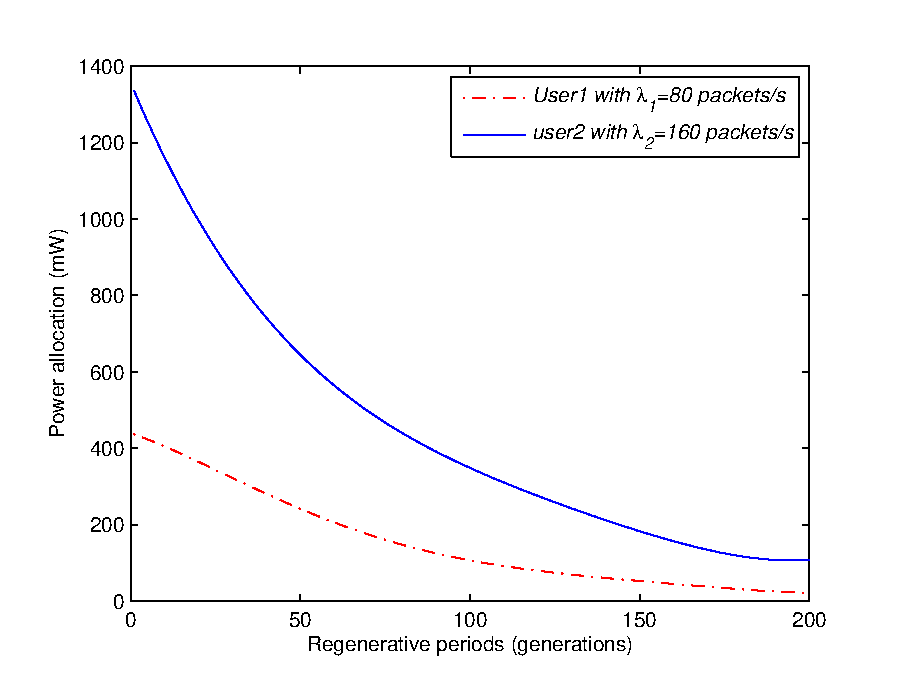
\includegraphics[width=3.5 in]{fig4.eps}
\vspace{-10pt}
\label{fig4}\caption{Average power expenditure versus regenerations periods of the two users.}
\end{figure}

\begin{figure}[htbt]
\centering
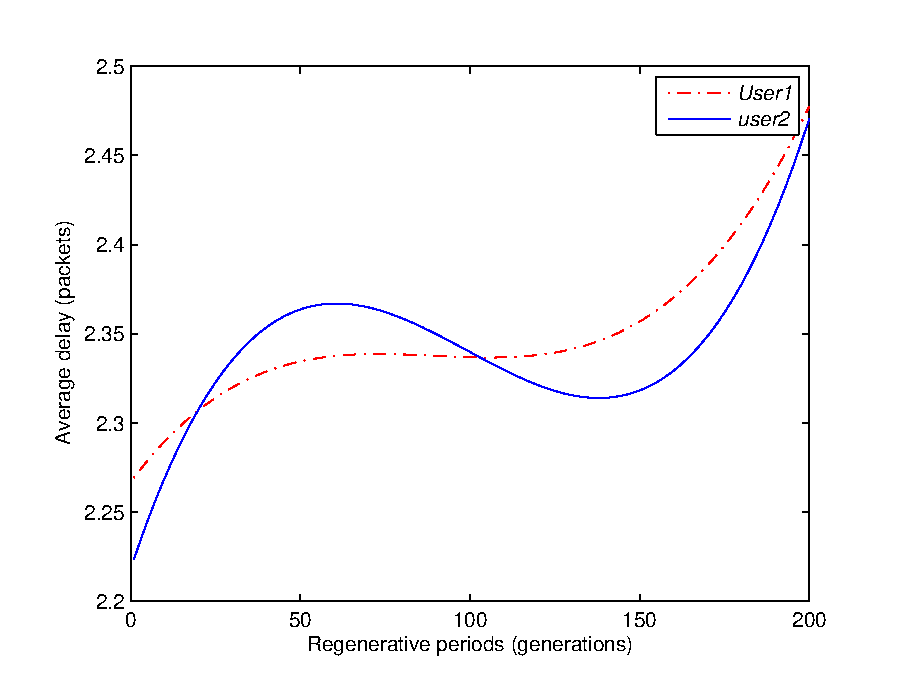
\includegraphics[width=3.5 in]{fig6.eps}
\vspace{-10pt}
\label{fig6}\caption{Average delay cost versus regenerations periods of the two users.}
\end{figure}

\begin{figure}[htbt]
\centering
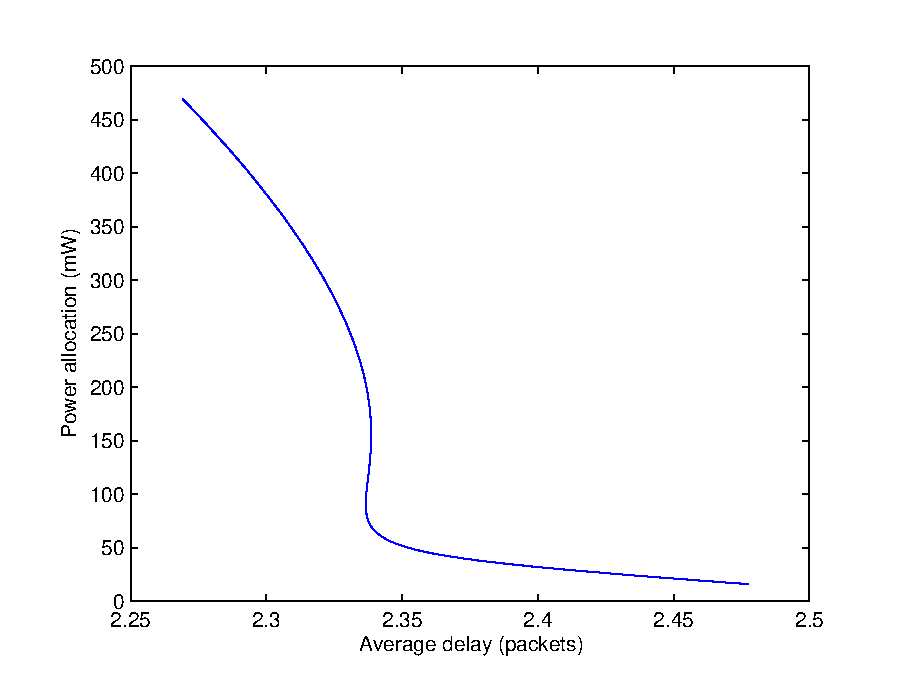
\includegraphics[width=3.5 in]{fig7.eps}
\vspace{-10pt}
\label{fig7}\caption{Average power allocation versus delay.}
\end{figure}

Fig. 2 depicts the trend of the norm of the post-decision state value function's different between two adjacent generations. As expected, it has a downward trend and an excellent allocation policy will be found if $\delta_v$ sets appropriated. Fig. 3 illustrates the average number of subcarriers varying with regenerations periods of the two users. Fig. 4 and Fig. 5 demonstrate the power expenditure and average delay cost varying with regenerations periods. In Fig. 4, the average power allocation has the similar trend with the norm of the post-decision state value function's difference that showed in Fig. 2. In Fig. 5, as the power allocation decreases, the average queue delay becomes higher. As the iteration number increases, we observe that the average power expenditure converges to a nearly fixed level. Fig. 6 illustrates the average power allocation versus delay with the regenerative periods. It verifies that the algorithm presents a significant energy reduction within average delay constraints. In practical applications, it is unnecessary to wait the algorithm to reach the convergence. Once the delay cost and the power expenditure fall in an acceptable region, it is reasonable to terminate the algorithm. It's not hard to find a feasible resource allocation scheme with low power requirement and non-homogenous delay constraint. Simulation results demonstrate that the algorithm converges to the optimal solution after the acceptable iterations almost surely.

\section{Conclusions}
In this paper, we conceive an energy-efficient power and subcarrier allocation scheme for downlink OFDMA systems under average delay constraints. The problem of dynamic power and subcarrier allocation is formulated as a CMDP with the control actions based on both CSI and QSI. We prove that the post-decision value function for the problem of the energy efficient scheduling under average delay constraint is convex on the backlog. We derive the equivalent state-reduced Bellman equation and propose an online stochastic value iteration solution to accelerate the algorithm convergence.

\bigskip

\begin{thebibliography}{13}

\bibitem{1} D. P. Bertsekas and R. Gallager, ``Data Networks'', \textit{Prentice Hall}, 1987.

\bibitem{2} R. A. Berry and R. G. Gallager, ``Communication over Fading
Channels with Delay Constraints,'' \textit{IEEE Transactions on
Information Theory}, Vol.48, No.5, pp.135-1149,2002.

\bibitem{3} H. Wang and N. Mandayam, ``A Simple Packet Transmission Scheme for
Wireless Data over Fading Channels,'' \textit{IEEE Transcations
on Communications}, Vol.52, No.7, pp.1055-1059, 2004.

\bibitem{4} M. Goyal, A. Kumar, and V. Sharma, ``Power Constrained and Delay Optimal
Policies for Scheduling Transmissions over a Fading Channel,'' \textit{Proceedings of IEEE INFOCOM}, Vol.1, pp.311-320, March.2003.

\bibitem{5} M. Agarwal, A. Karandikar, and V. S. Borkar, ``Structural Properties of
Optimal Transmission Policies over a Randomly Varying channel,''
Accepted for publication, \textit{IEEE Transactions on Automatic
Control}, 2007.

\bibitem{6} N. Salodkar, A. Karandikar, and V. S. Borkar, ``An On-Line
Learning Algorithm for Energy Efficient Delay Constrained Scheduling
over a Fading Channel,'' \textit{IEEE Journal on Selected Areas in
Com}, Vol.26, No.4, May.2008.

\bibitem{7} N. Salodkar, A. Karandikar, and V. S. Borkar, ``A Stable Online
Algorithm for Energy-Efficient Multiuser Scheduling,'' \textit{IEEE Transactions on mobile computing}, Vol.9, No.10, Oct.2010.

\bibitem{8} Fangwen Fu and Mihaela van der Schaar,'' Structure-Aware Stochastic
Control for Transmission Scheduling''.

\bibitem{9} Q. Zhang and S. A. Kassam, ``Finite-State Markov Model for
Rayleigh Fading Channels,'' \textit{IEEE Transactions on
Communications}, Vol.47, No.11, Nov.1999.

\bibitem{10}E. Altman, ``Constrained Markov decision processes: stochastic modeling,'' \textit{London: Chapman and Hall}, CRC, 1999.

\bibitem{11}A. Siem, D. Hertog and A. Hoffmann, ''A Method for Approximating Univariate Convex Functions Using Only Function Value Evaluations,''Online, available at SSRN:{http://ssrn.com/abstract=1012289}.

\bibitem{12}V. K. N. Lau and Y. Cui, "Delay-Optimal Power and Subcarrier Allocation for OFDMA Systems via Stochastic Approximation," \textit{IEEE Transactions on Wireless Communications}, Vol. 9, No.1, Jan.2010.
\end{thebibliography}


% that's all folks
\end{document}
